\documentclass{article}
\usepackage{geometry}
\geometry{a4paper, margin=1in}
\usepackage{graphicx}
\usepackage[colorlinks=true, linkcolor=blue, citecolor=blue, urlcolor=blue]{hyperref}
\usepackage{listings}
\usepackage{xcolor}
\usepackage{amsmath}
\usepackage{enumitem}
\usepackage{float}
\usepackage{subcaption}

\lstalias{none}{}

\lstset{
    language=Python,
    basicstyle=\ttfamily\footnotesize\selectfont, % use the selected monospaced font
    backgroundcolor=\color{white},
    keywordstyle=\color{blue},
    commentstyle=\color{gray},
    stringstyle=\color{red},
    numbers=left,
    numberstyle=\tiny\color{gray},
    stepnumber=1,
    numbersep=10pt,
    frame=single,
    breaklines=true,
    captionpos=b,
    tabsize=4
}

\title{Assignment 2 - Begging my Arduino to Blink \\
\large Why Tensorflow Why}
\author{
    [Welby Seely] \\
    \texttt{[wseely@emich.edu]}
}
\date{\today}

\begin{document}

    \maketitle


    \section{Two MLP Architectures}\label{sec:preamble}
    Modeled a Sine Wave With Two Different MLP Architectures.

    \subsection{Simple MLP Architecture}
    First up, a simple architecture with 2 fully connected layers, trained over 50 iterations.
    \\
    \begin{lstlisting}[label={lst:mlp1}]
        model = tf.keras.Sequential()
        model.add(keras.layers.Dense(10, activation='relu', input_shape=(1,)))
        model.add(keras.layers.Dense(1))
        model.compile(optimizer='adam', loss='mse', metrics=['mae'])
    \end{lstlisting}

    \begin{itemize}
        \item Basic model is 2488 bytes
        \item Quantized model is 3040 bytes
        \item Difference is -552 bytes
    \end{itemize}

    \begin{figure}[!htbp]
        \centerline{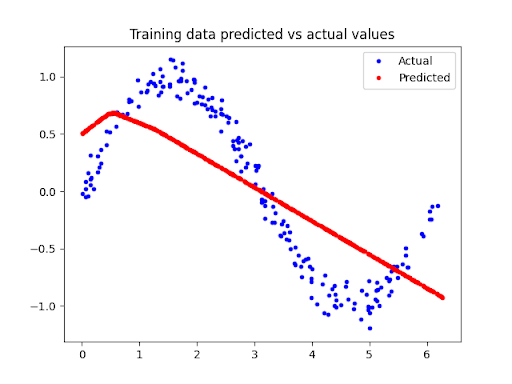
\includegraphics[width=0.8\columnwidth]{simple}}
        \caption{Simple MLP Network}
        \label{fig:simplemlp}
    \end{figure}

    ReLu in a single layer does not allow for a great approximation of the Sine wave.
    Quantized model size was 552 bytes larger than the original due to quantized model metadata.

    \subsection{More Complex MLP Architecture}
    Second, a more complex architecture with 5 fully connected layers, trained over 500 iterations.
    Still using ReLu as the activation function.

    \\
    \begin{lstlisting}[label={lst:mlp2}]
        model = tf.keras.Sequential()
        model.add(keras.layers.Dense(16, activation='relu', input_shape=(1,)))
        model.add(keras.layers.Dense(16, activation='relu'))
        model.add(keras.layers.Dense(128, activation='relu'))
        model.add(keras.layers.Dense(16, activation='relu'))
        model.add(keras.layers.Dense(1))
        model.compile(optimizer='adam', loss="mse", metrics=["mae"])
    \end{lstlisting}

    \begin{figure}[!htbp]
        \centerline{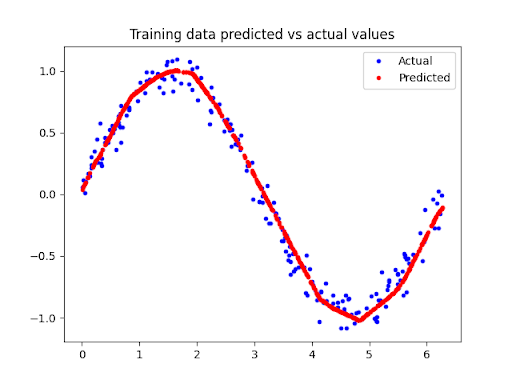
\includegraphics[width=0.8\columnwidth]{complex}}
        \caption{A More Complex MLP Network}
        \label{fig:complex}
    \end{figure}

    \begin{itemize}
        \item Basic model is 20932 bytes
        \item Quantized model is 8720 bytes
        \item Difference is 12212 bytes
    \end{itemize}

    With multiple layers, ReLu can better approximate the non-linearity of the Sine wave.
    The compressed model size is noticeable with a network of this size.

    \section{Angrily Staring at a Light that Refuses to Blink }\label{sec:arduino}

    Deployed models did not exhibit the expected behavior of the networks.
    Switched to using quantized inputs:

    \begin{lstlisting}[label={lst:qin}]
    converter.target_spec.supported_ops = [tf.lite.OpsSet.TFLITE_BUILTINS_INT8]
    converter.inference_input_type = tf.int8  # Optional: Omit to keep I/O as float
    converter.inference_output_type = tf.int8  # Optional: Omit to keep I/O as float
    \end{lstlisting}

    Updated the Arduino loop accordingly:

    \begin{lstlisting}[label={lst:aloop}]
          int8_t x_quantized = x / input->params.scale + input->params.zero_point;
          input->data.int8[0] = x_quantized;
    \end{lstlisting}

    After an initial test where the results almost looked reasonable, retraining and redeploying proved that there was no change in the inaccuracies.

    To debug, I first added more extensive logging to the application just to make sure I understood the data correctly:

    \begin{lstlisting}[label={lst:print}]
    \end{lstlisting}

    Each time I would train a network, I would get wildly different results.
    It couldn't be due to normal quantization errors - the results were just plain wrong.

    I figured this had to be due to something going wrong when converting the model to TFLite and quantizing, since the model validation and test data points proved the models were adequate/reasonable.

    Verified the model using the TFLite interpreter in the same code that trained the models.

    \begin{lstlisting}[label={lst:quant}]
    def predict(x_data):
      predictions = []
      for x in x_data:
        # Set the input tensor
        interpreter.set_tensor(input_details[0]['index'], np.array([[x]], dtype=np.float32))
        interpreter.invoke()
        # Get the output tensor
        output = interpreter.get_tensor(output_details[0]['index'])
        predictions.append(output[0][0])
      return np.array(predictions)

    interpreter = tf.lite.Interpreter(model_path=f"{MODELS_DIR_RELATIVE}/sine_model_quantized.tflite")
    interpreter.allocate_tensors()

    input_details = interpreter.get_input_details()
    output_details = interpreter.get_output_details()

    nonquantized_predictions = model.predict(x_test)
    quantized_predictions = predict(x_test)
    plt.figure(figsize=(10, 6))
    plt.title('Quantized Model Predictions vs Actual Values')
    plt.plot(x_test, y_test, 'b.', label='Actual')
    plt.plot(x_test, nonquantized_predictions, 'g.', label='Model Prediction')
    plt.plot(x_test, quantized_predictions, 'r.', label='Quantized Model Prediction')
    plt.legend()
    plt.xlabel('x')
    plt.ylabel('y')
    plt.show()
    \end{lstlisting}

    \begin{figure}[!htbp]
        \centerline{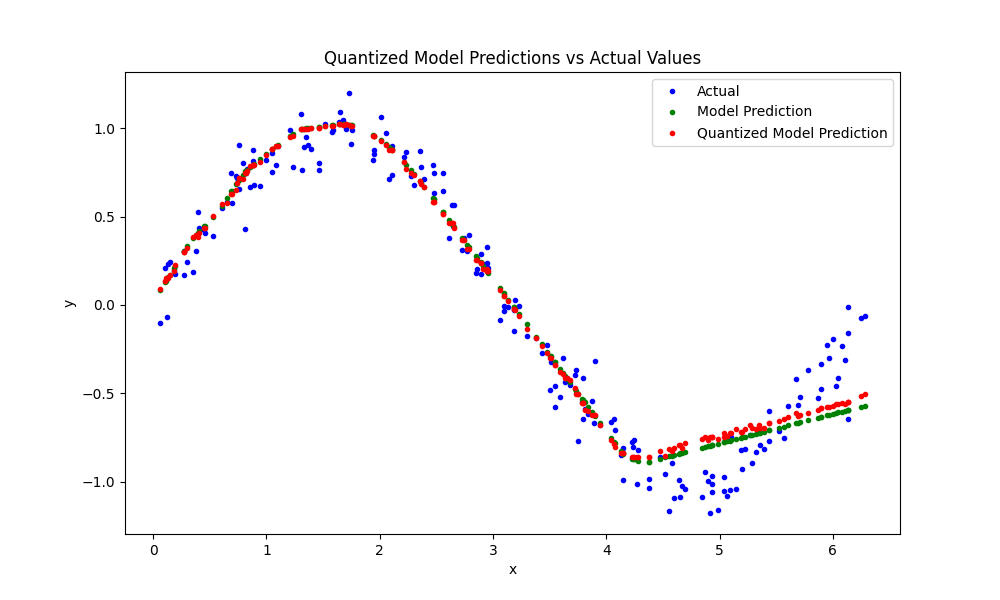
\includegraphics[width=0.8\columnwidth]{quantized}}
        \caption{Model vs Quantized Model}
        \label{fig:quantized}
    \end{figure}

    The quantized model is working perfectly satisfactorily.
    This means that the likely culprit is that the quantized model binary produced by Tensorflow 2.18.1 (the version I was using) is not compatible with the version used by TensorFlow Lite Micro Arduino Examples~\cite{tfliteMicroArduino}.
    Unfortunately, the authors of the examples failed to document the version of TFLite that they were using.

    I briefly looked into updating the TFLite library used in Arduino Examples - the library is customized for Arduino, so I couldn't just plop a new version in its place.
    Updating it was feasible if I didn't have anything else to do with my life, but I figured now is not the time to devote myself to Tensorflow on Arduino.

    So, I looked into downgrading the version Tensorflow used to train the models.
    Downgraded to Tensorflow 2.12.0, the earliest version supported by Python 3.11 (the runtime I was working with on that particular machine).
    I retrained the model, uploaded to the Arduino and\ldots voilà!
    It worked!
    Through trial and error I discovered that 2.15.1 was the latest version that worked both on my machine and with the Arduino.
    2.16.x produced weird errors when converting to TFLite, so I didn't even get to test that on the Arduino board.

    \subsection{What did Tensorflow change?}\label{subsec:what-did-tensorflow-change?}

    A number of changes to TFLite were introduced in Tensorflow 2.17.x, including changes to quantization behavior and a Flatbuffer update~\cite{tensorflow2.17.0}.
    This is the likely cause of model incompatibility with earlier versions of Tensorflow.
    I'm not sure why Tensorflow 2.16.x errored out, but I don't believe it was the version that introduced this incompatibility.

    \subsection{Did the light finally blink?}\label{subsec:did-the-light-finally-blink?}

    At long last, after many lamentations, in the face of tremendous trials and tribulations\ldots the light indeed blinked.
    It made a smooth transition in the complex model, and awkwardly jumped from off to on in the simple model, just as was expected.

    \subsection{Make The Light Blink Faster}\label{subsec:make-the-light-blink-faster}

    The light can be made to blink faster in at least four different ways:

    \begin{enumerate}
        \item Train a new model with a higher frequency across the same $2\pi$ domain.
        \item Update the delay in arduino\_output\_handler.cpp.
        \item Update the kInferencesPerCycle in arduino\_constants.cpp.
        \item Use the latest version of Tensorflow, pick a god and pray.
    \end{enumerate}

    Here's an example of the delay being updated, changed from 33 to 16 milliseconds (roughly doubling frequency):

    \begin{lstlisting}[label={lst:delay}]
    void HandleOutput(float x_value, float y_value) {
      if (!initialized) {
        // Set the LED pin to output
        pinMode(led, OUTPUT);
        initialized = true;
      }

      int brightness = (int)(127.5f * (y_value + 1));

      int brightness_clamped = std::min(255, std::max(0, brightness));

      analogWrite(led, brightness_clamped);

      MicroPrintf("%d\n", brightness_clamped);
      delay(16); // this is the only thing I updated
    }
    \end{lstlisting}

    \section{Github Repo}\label{sec:deliverables}
    My messy repo can be found here \href{https://github.com/crimsonmagick/cosc592\_arduino1.git}{here on Github}.

    \bibliographystyle{plainurl}
    \bibliography{bibliography}
\end{document}
